\section{结果评价}
\label{sec:minimax-evaluation}

算法停下来，交出一对$(\bm{x},\bm{y})$，它有多好？极小极大问题里，$f(\bm{x}^{(t)},\bm{y}^{(t)})$的升降不能回答这个问题，图~\ref{fig:minimax-gda-monitor}已经表明，两侧的优化方向本来相反，这个数上下波动没有确定的含义。

所以第一步是说清要评价什么。表~\ref{tab:minimax-evidence}按目标列出相应的证据。

\begin{BookInlineTable}
 \centering
 \begin{tabular}{@{}lll@{}}
  \toprule
  目标 & 证据 & 成立前提\\
  \midrule
  全局鞍点 & 间隙$G$或其有效上界 & 两侧极值能算或能界\\
  值函数最小 & $\phi$的（次）梯度 & 内层响应可信\\
  局部结构 & 二阶条件 & 只在邻域内有意义\\
  \bottomrule
 \end{tabular}
 \caption{评价目标与相应的证据。}
 \label{tab:minimax-evidence}
\end{BookInlineTable}

\subsection{误差证据}
\label{sec:minimax-error-evidence}

凸凹问题上最好的证据是间隙~\eqref{eq:minimax-gap}。若$\phi$和$\psi$能直接算出，例如$f$双线性而$\bm{X},\bm{Y}$是单纯形或盒子，内层就是线性函数在顶点上取值，这时间隙是精确的。

\paragraph{平均点与最后一点}
定理~\ref{thm:minimax-eg-gap}保证的是平均点。最后一点可能完全不同。在盒子$[-1,1]^2$上，$f=xy$，$L=1$，取外梯度法的边界步长$\alpha=1$，从$(1,0)$出发。第一轮试探点和校正点是
\[
 \tilde{\bm{z}}^{(0)}=(1,1),\qquad\bm{z}^{(1)}=(1,0)-(1,-1)=(0,1).
\]
继续下去，$\bm{z}^{(t)}$依次经过$(1,0),(0,1),(-1,0),(0,-1)$，每四轮回到起点。试探点依次是四个顶点。

由式~\eqref{eq:minimax-box-gap}，最后一点的间隙恒为$1$，没有收敛。而试探点的平均，$T=1,2,3,4$时间隙分别是$2,1,\frac23,0$，都不超过定理的上界$\frac{D^2}{2\alpha T}=\frac4T$，这里$D^2=8$，见图~\ref{fig:minimax-average-last}。

\begin{BookInlineFigure}
 \centering
 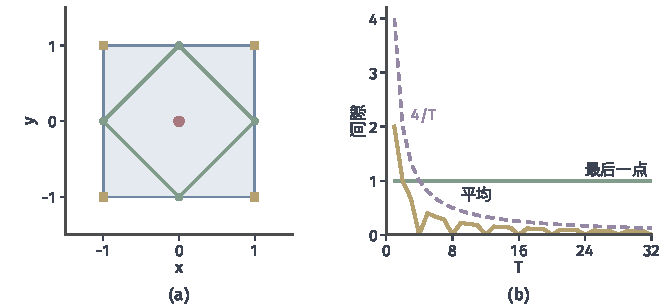
\includegraphics[width=112mm]{figures/05-optimization/07-multiple-criteria-and-nested-optimization/matplotlib/minimax-average-last/figure.pdf}
 \caption{外梯度法取边界步长$\alpha=1/L=1$，$f=xy$，$\bm{Z}=[-1,1]^2$，起点$(1,0)$。(a)绿点是校正点，沿菱形循环；黄色方块是试探点，在四个顶点循环；红点是鞍点。(b)绿线是最后一点的间隙，恒为$1$；黄线是试探点平均的间隙，在每四轮的整数倍处为$0$；紫色虚线是上界$4/T$。}
 \label{fig:minimax-average-last}
\end{BookInlineFigure}

$\alpha<1/L$时可以证明校正点本身收敛到某个鞍点，这个例子的循环出现在边界步长上。最后一点的间隙速率比平均点慢，一般是$O(1/\sqrt{T})$，证明较长，读者可查阅外梯度法最后迭代分析的专门文献。报告结果时要说清楚输出的是平均点还是最后一点，因为定理的结论只属于它所针对的那一个。

\paragraph{近似内层给出的间隙偏小}
$\phi$和$\psi$算不出来时，通常用内层算法分别求一个近似响应$\tilde{\bm{y}}$和近似外层点$\tilde{\bm{x}}$，然后计算
\begin{equation}
 \hat{G}=f(\bm{x},\tilde{\bm{y}})-f(\tilde{\bm{x}},\bm{y}).
 \label{eq:minimax-gap-estimate}
\end{equation}

因为$f(\bm{x},\tilde{\bm{y}})\leq\phi(\bm{x})$，$f(\tilde{\bm{x}},\bm{y})\geq\psi(\bm{y})$，所以$\hat{G}\leq G$。这与第~\ref{chap:duality}章“内层近似的方向”是同一个现象，误差方向正好不利：内层算得越粗糙，估计的间隙越小，算法看起来越好。

取盒子上的$f=xy$，候选$(x,y)=(0.4,-0.2)$，由式~\eqref{eq:minimax-box-gap}，真实间隙是$0.6$。内层只走一步步长$\frac12$的投影梯度：
\[
 \tilde{y}=-0.2+\frac12\cdot0.4=0,\qquad\tilde{x}=0.4-\frac12\cdot(-0.2)=0.5.
\]
式~\eqref{eq:minimax-gap-estimate}给出
\[
 \hat{G}=f(0.4,0)-f(0.5,-0.2)=0+0.1=0.1.
\]
真实间隙$0.6$被低估了六倍。

要得到可靠的上界，必须把内层误差补回去。第~\ref{chap:duality}章由梯度残差得到认证界：$\mu$强凸函数在$\tilde{\bm{x}}$处的最小值至少是函数值减去$\lVert\nabla\rVert_2^2/(2\mu)$。把它用到$-f(\bm{x},\cdot)$和$f(\cdot,\bm{y})$上。设$\bm{X}=\mathbb{R}^n$，$\bm{Y}=\mathbb{R}^q$，$f(\bm{x},\cdot)$是$\mu_y$强凹的，$f(\cdot,\bm{y})$是$\mu_x$强凸的，则
\begin{equation}
 G(\bm{x},\bm{y})\leq\hat{G}+\frac{\lVert\nabla_{\bm{y}}f(\bm{x},\tilde{\bm{y}})\rVert_2^2}{2\mu_y}+\frac{\lVert\nabla_{\bm{x}}f(\tilde{\bm{x}},\bm{y})\rVert_2^2}{2\mu_x}.
 \label{eq:minimax-certified-gap}
\end{equation}

验算一例。$f=\frac12x^2+2xy-\frac12y^2$，$\mu_x=\mu_y=1$，候选$(0.2,0.1)$。真实值由$\phi(x)=\frac52x^2$，$\psi(y)=-\frac52y^2$算出，
\[
 G=0.1+0.025=0.125.
\]

取近似响应$\tilde{y}=0.3$，$\tilde{x}=-0.1$，则
\[
 f(0.2,0.3)=0.095,\qquad f(-0.1,0.1)=-0.02,\qquad\hat{G}=0.115.
\]
两个残差是$\partial_yf(0.2,0.3)=0.1$，$\partial_xf(-0.1,0.1)=0.1$，式~\eqref{eq:minimax-certified-gap}的修正量各是$0.005$，得到上界
\[
 0.115+0.005+0.005=0.125.
\]
未修正的$\hat{G}$比真实间隙小，修正之后的上界不小于真实间隙。这里等号成立，因为函数恰好是二次的，曲率常数处处精确。

\subsection{非凸问题}
\label{sec:minimax-nonconvex}

没有凸凹性时，间隙可能恒为正，甚至恒为无穷，图~\ref{fig:minimax-saddle-types}(c)的原点就是这样。此时的目标是顺序问题本身，证据要分三层报告，各说明它证明了什么。

\paragraph{值函数的驻定证据}
内层强凹时，$\phi$可微，外层的驻定量可以由已知量给出上界。由三角不等式和式~\eqref{eq:minimax-gradient-error}，
\begin{equation}
 \lVert\nabla\phi(\bm{x})\rVert_2\leq\lVert\nabla_{\bm{x}}f(\bm{x},\tilde{\bm{y}})\rVert_2+L\sqrt{\frac{2\varepsilon}{\mu}}.
 \label{eq:minimax-stationarity-bound}
\end{equation}

用$f=-\frac12x^2+2xy-\frac12y^2$，取$x=0.1$，$\tilde{y}=0.18$。此时外层偏导数是$-0.1+0.36=0.26$，内层间隙是$\frac12(0.02)^2=0.0002$。交叉系数是$2$，第二项是$2\cdot0.02=0.04$，上界是$0.30$，真实导数$3x$也是$0.30$。

式~\eqref{eq:minimax-stationarity-bound}需要$\varepsilon$的可靠上界。内层强凹且无约束时，式~\eqref{eq:minimax-certified-gap}用到的残差界同样适用，$\varepsilon$不超过残差平方除以$2\mu$；有约束时要用相应的对偶界。

\paragraph{响应求解的证据}
内层不凹时，$\varepsilon$一般没有可计算的上界。从多个起点运行内层算法，取最大的值作为$\phi(\bm{x})$的估计，这是一个越算越大的下界。报告时要写成“在所检查的响应中最坏值是多少”，并说明检查的范围。它不是全局最坏值。式~\eqref{eq:minimax-nonconcave}在$x=1$处，从$y<-0.618$出发只能得到$0.25$，从$y>-0.618$出发才能得到$3.023$。

\paragraph{局部极小极大条件}
不要求全局最坏时，可以问一个更弱的问题：相对于局部的响应分支，当前点是不是极小？下面的二阶充分条件给出一种准确的说法。

\begin{theorem}[局部极小极大的二阶充分条件]
\label{thm:minimax-local}
设$f$在$(\bar{\bm{x}},\bar{\bm{y}})$附近二阶连续可微，$\nabla_{\bm{x}}f$和$\nabla_{\bm{y}}f$在该点为零，$\nabla^2_{\bm{y}\bm{y}}f\prec\bm{0}$，并且
\begin{equation}
 \bm{S}=\nabla^2_{\bm{x}\bm{x}}f-\nabla^2_{\bm{x}\bm{y}}f\,(\nabla^2_{\bm{y}\bm{y}}f)^{-1}\,\nabla^2_{\bm{y}\bm{x}}f\succ\bm{0}.
 \label{eq:minimax-schur}
\end{equation}
则存在定义在$\bar{\bm{x}}$某邻域上的连续可微映射$\bm{y}(\bm{x})$，$\bm{y}(\bar{\bm{x}})=\bar{\bm{y}}$，使$\bm{y}(\bm{x})$是$f(\bm{x},\cdot)$的局部极大点，且$\bar{\bm{x}}$是$\bm{x}\mapsto f(\bm{x},\bm{y}(\bm{x}))$的严格局部极小点。称这样的$(\bar{\bm{x}},\bar{\bm{y}})$为\term{局部极小极大点}（local minimax point）。
\end{theorem}

\begin{proof}
方程$\nabla_{\bm{y}}f(\bm{x},\bm{y})=\bm{0}$在该点关于$\bm{y}$的Jacobian是$\nabla^2_{\bm{y}\bm{y}}f$，可逆。隐函数定理给出连续可微的$\bm{y}(\bm{x})$，其导数是
\[
 \nabla\bm{y}(\bm{x})=-(\nabla^2_{\bm{y}\bm{y}}f)^{-1}\nabla^2_{\bm{y}\bm{x}}f.
\]
由连续性，$\nabla^2_{\bm{y}\bm{y}}f$在邻域内保持负定，所以$\bm{y}(\bm{x})$是局部极大点。

令$h(\bm{x})=f(\bm{x},\bm{y}(\bm{x}))$。因为在响应分支上$\nabla_{\bm{y}}f=\bm{0}$，链式法则只留下关于$\bm{x}$的偏梯度：
\[
 \nabla h(\bm{x})=\nabla_{\bm{x}}f(\bm{x},\bm{y}(\bm{x})).
\]
再求一次导，得到
\[
 \nabla^2h=\nabla^2_{\bm{x}\bm{x}}f+\nabla^2_{\bm{x}\bm{y}}f\,\nabla\bm{y}(\bm{x}).
\]
代入$\nabla\bm{y}$的表达式，在$\bar{\bm{x}}$处就是$\bm{S}$。又$\nabla h(\bar{\bm{x}})=\bm{0}$，$\bm{S}\succ\bm{0}$，由二阶充分条件，$\bar{\bm{x}}$是$h$的严格局部极小点。
\end{proof}

对$f=-\frac12x^2+2xy-\frac12y^2$，$\nabla^2_{yy}f=-1$，$S=-1-2\cdot(-1)\cdot2=3$，恰好是$\phi''$。

这个条件只回答局部响应分支。把式~\eqref{eq:minimax-nonconcave}放到$(1,-1)$处，两个偏导数$x+y$和$x+2y-y^3$都是$0$，$\partial_y^2f=2-3y^2=-1<0$，$\partial_x^2f=1$，$\partial_{xy}f=1$，
\[
 S=1-1\cdot(-1)\cdot1=2>0.
\]
定理的全部条件都满足，$(1,-1)$是局部极小极大点。可是$\phi'(1)=2.618\neq0$，$\phi(1)=3.023$，而外层真正的最优解是$x=0$。局部极小极大是相对于“内层只能看到附近”这个模型的结论，不能当作原问题的解来报告。

\paragraph{计算预算}
不同方法每轮的工作量相差悬殊，一轮精确内解和一轮下降—上升不能直接比较。图~\ref{fig:minimax-budget}是同一组运行的两种画法。(a)按外层轮数，$K=1$明显落后，$K=10$几乎与精确响应重合，$K=3$在这组系数下收缩最快；(b)按梯度读取总数，$K=10$反而最慢，因为它每轮要读$11$次。

\begin{BookInlineFigure}
 \centering
 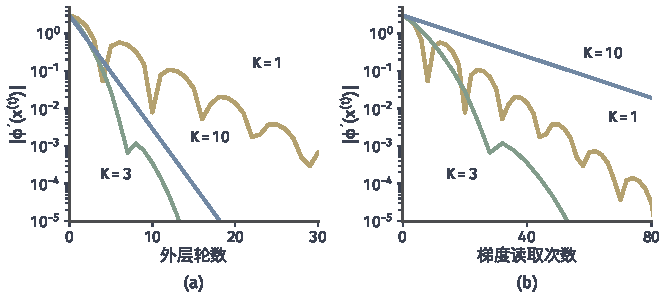
\includegraphics[width=112mm]{figures/05-optimization/07-multiple-criteria-and-nested-optimization/matplotlib/minimax-budget/figure.pdf}
 \caption{$f=-\frac12x^2+2xy-\frac12y^2$上每轮做$K$步内层上升的方法，$\alpha=\frac16$，$\beta=\frac12$，起点$(1,0)$。黄线$K=1$，绿线$K=3$，蓝线$K=10$。(a)按外层轮数，灰色虚线是精确响应。(b)同样的运行按梯度读取次数，每轮读取$K+1$次。}
 \label{fig:minimax-budget}
\end{BookInlineFigure}

报告的预算应当分开写明外层迭代次数、每次内层的计算量以及方向读取的总次数。这个例子里内层便宜且条件好，$K=3$在读取次数上最省。换一个问题，这个顺序可以完全不同。
